\begin{quote}
    \textit{``Roger (Penrose) noticed something very interesting about the signs of these guys. ...well, I have no idea if that was actually the case, I'm just making this up as I go along.'' --Jorge Santos}
\end{quote}
We showed last time that we can characterize the behavior of null congruences by three objects-- the expansion, the shear, and the rotation. Having showed that the rotation was zero under certain conditions, we now consider the consequences of these objects.

\subsection*{Gaussian null coordinates} For a null hypersurface $\mathcal{N}$, take a $2$D spacelike surface $S$ with coordinates $y_i$ on $\mathcal{N}(U)$. Take another null vector field $V$ on $\mathcal{N}$ satisfying \begin{equation}
    V\cdot \P{}{y^i}=0\text{ and } V\cdot U=1, V^2=0.
\end{equation}
Now we assign coordinates $(r,\lambda,y^i)$ to the point at affine parameter distance $r$ along the null geodesic which starts at the point on $\mathcal{N}$ with coordinate $(\lambda,y^i)$ and has tangent vector $V^a$. Thus we follow $U$ along $\mathcal{N}$ $(r=0)$ for distance $\lambda$ and then go off $\mathcal{N}$ by following $V$ for affine parameter $r$. See Fig. \ref{fig:gaussiannullcoords} for an illustration.

\begin{figure}
    \centering
    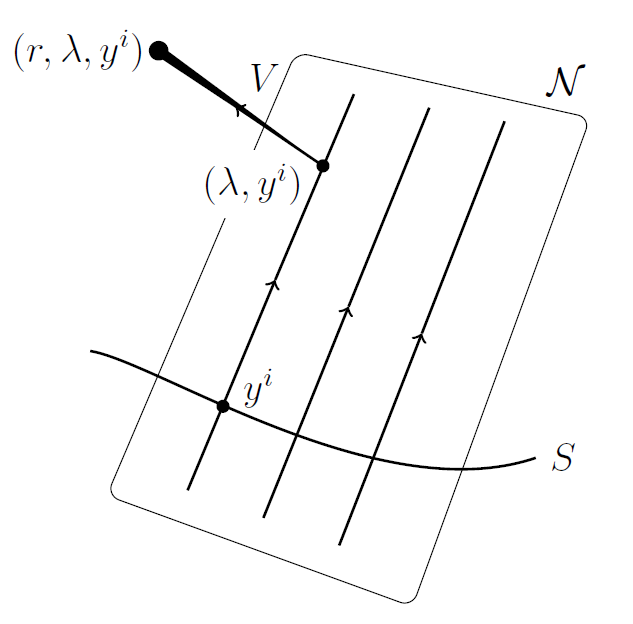
\includegraphics{2019/02/20190220_reall_gaussiannullcoords.png}
    \caption{An illustration of Gaussian null coordinates. For a null hypersurface $\cN$, take a 2D spacelike surface $S\subset \cN$ with coordinates $y_i$. We construct the integral curves of $U$ (the generators of $\cN$) and from $S$, follow these curves for affine parameter distance $\lambda$. Finally, we take a null vector field $V$ and follow its integral curves off of $\cN$ for a distance $r$.\newline
    %
    Image credit to Prof. Reall's  \href{http://www.damtp.cam.ac.uk/user/hsr1000/black_holes_lectures_2016.pdf}{Black Holes notes}, \textsection 4.6.
    }
    \label{fig:gaussiannullcoords}
\end{figure}

This defines a coordinate chart in a neighborhood of $\mathcal{N}$ such that the hypersurface $\mathcal{N}$ is at $r=0$, with $U=\P{}{\lambda}$ on $\mathcal{N}$ and $\P{}{r}$ tangent to affinely parametrized null geodesics.

The latter condition implies that $g_{rr}=0$ everywhere (that is, $g_{\mu\nu}(\P{}{r})^\mu (\P{}{r})^\nu = g_{rr}=0$). It also follows from the geodesic equation for $\P{}{r}$ that
\begin{equation}
    g_{r\mu,r}=0,
\end{equation}
where $\mu$ is now a free index that runs over $r,\lambda,y^i$.%
    \footnote{The proof is left as an exercise in Harvey Reall's notes. It's two lines: let $U^\mu=(1,0,0,0)$ in $(r,\lambda,y^1,y^2)$ coordinates. Then the geodesic equation says that
    \begin{align*}
        0&=\frac{d U^\mu}{d\tau} + \Gamma^\mu_{\alpha\beta} U^\alpha U^\beta\\
            &=\Gamma^\mu_{rr} = g^{\mu\sigma}(g_{r\sigma,r}+ g_{\sigma r,r} - g_{rr,\sigma}) = 2g^{\mu\sigma}g_{r\sigma,r}
    \end{align*}
    since $g_{rr}=0$ and $g$ is symmetric. We conclude that $g_{r\sigma,r}=0$ for any index $\sigma$.
    }
%
But at $r=0$, we have $g_{r\lambda}=U\cdot V = 1$, and $g_{ri}=V\cdot \P{}{y^i}=0$.
So these are the first indications these are good coordinates. We also know that $g_{\lambda\lambda}=0$ at $r=0$, as $U^a$ is null, and $g_{\lambda i}=0$ at $r=0$, as $\P{}{y^i}$ is tangent to $\mathcal{N}$ and hence orthogonal to $U^a$. Thus the metric components take the form
\begin{equation}
    g_{\lambda\lambda}= rF, \quad g_{\lambda i} = r h_i,
\end{equation}
and we find the metric in these coordinates takes the form
\begin{equation}
    ds^2 = 2drd\lambda +rF d\lambda^2 +2rh_i d\lambda dy^i + h_{ij} dy^i dy^j.
\end{equation}

Note that at $r=0,$ $F$ must vanish. To see this, we use the fact that
\begin{equation}
     \lambda\mapsto (0,\lambda,y^i)
\end{equation}
are affinely parametrized null geodesics. For this, the only non-vanishing component of the geodesic equation is the $r$ component,
\begin{equation}
    \p_r (rF)=0.
\end{equation}
Integrating this at $r=0$ tells us that $F=0$ at $r=0$, so we can write $F=r\hat F$ for $\hat F$ some smooth function. WLOG we can therefore write
\begin{equation}
    ds^2 = 2drd\lambda +r^2 \hat F d\lambda^2 +2rh_i d\lambda dy^i + h_{ij} dy^i dy^j.
\end{equation}

What does this metric look like on our null hypersurface? On $\mathcal{N}$, the metric is simply
\begin{equation}\label{nullhsurfacemetric}
    g|_{\mathcal{N}}= 2drd\lambda +h_{ij} dy^i dy^j.
\end{equation}
Thus $U^\mu=(0,1,0,0)$ on $\mathcal{N}$, which implies $U_\mu=(1,0,0,0)$ (where we've lowered the index using $g|_{\mathcal{N}}$). Recall that 
\begin{equation}
    U\cdot B = B\cdot U=0 \implies B^r{}_\mu = B^\mu{}_\lambda = 0.
\end{equation}
We also know that $\theta=B^\mu{}_\mu$, but we've just shown that two of the trace components vanish, $B^r{}_r=B^\lambda{}_\lambda=0$, so it must be the $y^i$ components which contribute to the expansion. On $\mathcal{N},$
\begin{align}
    \theta = B^i{}_i &=\nabla_i U^i = \p_i U^i +\Gamma^i_{i\mu} U^\mu\\
    &= \Gamma^i_{i \lambda} =\frac{1}{2} h^{ij}(g_{ji,\lambda} + g_{j\lambda,i}-g_{i\lambda,j})\\
    &=\frac{1}{2} h^{ij}h_{ji,\lambda}\\
    &= \frac{\p_\lambda\sqrt{h}}{\sqrt{h}}
\end{align}
where $h=\det h_{ij}$. To make the simplifications in the first and second lines, we notice that $\p_i U^i=0$ and $g_{i\lambda}=0$ on $\cN$ (remark: $\lambda$ is a component, not a free index!). Hence we have
\begin{equation}
    \frac{d\sqrt{h}}{d\lambda} = \theta \sqrt{h}.
\end{equation}
Borrowing a notation from Witten, if we denote $V\equiv \sqrt{h}$, then $\theta = \dot V/V$. Since $V$ represents the volume of a little area on $S$, $\theta$ represents the normalized expansion of that volume as we flow along the null geodesics in the congruence.

\subsection*{Trapped surfaces}
%We're warming up now, because the next class will be *the* most difficult class.
Consider a 2D spacelike surface $S$, i.e. a 2D submanifold for which all tangent vectors are spacelike. For any $p\in S$, there will be \emph{precisely} two future-directed null vectors $U^a{}_1, U^a{}_2$ orthogonal to $S$ (up to a freedom of rescaling).%
    \footnote{``If you want to see if you really understand the class, go home and think about why the word precisely is here.''}
This generalizes the notion of ingoing and outgoing trajectories.
\begin{exm}
    Let $S$ be a 2-sphere with $U=U_0,V=V_0$ in the Kruskal spacetime. (That is, points in the Kruskal diagram represent 2-spheres.) By spherical symmetry, the generators of $\mathcal{N}_i$ will be radial null geodesics.
    %diagram
    Hence, $\mathcal{N}_i$ must be surfaces of constant $U$ or constant $V$, with the generators tangent to $dU$ and $dV$. Raising the index, we have
    \begin{equation}
        U^a{}_1 = re^{r/2M} \paren{\P{}{V}}^a,\quad U^a{}_2 = re^{r/2M} \paren{\P{}{U}}^a.
    \end{equation}
    We have fixed signs such that both are future-directed. Now
    \begin{gather}
        \theta_1 = \nabla_a U^a{}_1 = \frac{1}{\sqrt{g}}\p_a(\sqrt{-g} U^a{}_1) =-\frac{8M^2}{r} U,\\
        \theta_2 = -\frac{8M^2}{r}V.
    \end{gather}
    But note that $U$ and $V$ have different signs in the different quadrants of the Kruskal diagram. Something very interesting happens because of this.
    %Roger (Penrose) noticed something very interesting about the signs of these guys. ...well, I have no idea if that was actually the case, I'm just making this up as I go along.
    
    For $S$ in region I, we have
    \begin{equation}
        U <0, V > 0 \implies \theta_1 >0, \theta_2 <0.
    \end{equation}
    Region IV is similar. But region II (the black hole interior) is different. Here,
    \begin{equation}
        U>0, V>0 \implies \theta_1 <0, \theta_2 <0,
    \end{equation}
    so now both the expansion coefficients are negative, and everything is shrinking as we flow along congruences.
\end{exm}
\begin{defn}
    A compact orientable 2D spacelike surface is \term{trapped} if both families of null geodesics orthogonal to $S$ have negative expansion everywhere on $S$.
\end{defn}
As it turns out, the existence of trapped surfaces is closely related with the presence of singularities-- they are a condition in the famous Penrose singularity theorems.

\subsection*{The Raychaudhuri equation}
\begin{prop}
    With the expansion defined as before,
    \begin{equation}
        \frac{d\theta}{d\lambda}=-\frac{1}{2} \theta^2 +\hat\sigma^{ab} \hat\sigma_{ab}+\hat \omega^{ab} \hat \omega_{ab} - R_{ab} U^a U^b.
    \end{equation}
    %I stress this is simple. And yet it has absolutely fascinating consequences.
\end{prop}
\begin{proof}
    We start out with
    \begin{align*}
        \frac{d\theta}{d\lambda} &= U\cdot \nabla (B^a{}_b P^b{}_a)\\
        &= P_a{}^b U \cdot \nabla B^a{}_b\\
        &= P_a{}^b U^c (\nabla_c \nabla_b U^a+R^a{}_{dcb}U^d)\\
        &= P_a{}^b \bkt{\nabla_b(U^c\nabla_c U^a)-(\nabla_b U^c)(\nabla_c U^a)
        }+P_a{}^b R^a{}_{dcb} U^c U^d\\
        &= -B^c{}_b P^b{}_a B^a{}_c -R_{cd} U^c U^d\\
        &= -\hat B^c{}_a \hat B^a{}_c - R_{ab} U^a U^b.
    \end{align*}
    where we've used the Ricci identity to commute the derivatives and moved a $U$ inside a derivative with Leibniz in order to get something that vanishes by the geodesic equation.
    
    Instead of just $B^2$, we've got $\hat B^2$, which is even nicer, and from here we simply insert the explicit expression for $\hat B$ in terms of $\theta,\hat \sigma,$ and $\hat \omega$.
\end{proof}
But notice that none of this proof depends on the Einstein equations! It can be formulated as a purely geometric statement. Where Einstein comes in is in recognizing that the Ricci tensor has appeared in the Raychaudhuri equation, and in particular the Einstein equations connect the Ricci tensor to the stress tensor. $R_{ab}U^a U^b$ is some contracted quantity, and what this starts to suggest to us is conditions on the matter that lives in spacetime, i.e. energy conditions.